% questions.tex —— 2016 年·春季上海卷 · 题目内容片段（无答案）
% 由 tools/generate_projects.py 依来源总账自 2016/2016_数学真题_春季上海_试题.md 生成，勿手改（改源 MD 后重跑）


\gkpart{数学}

\begin{gktip}
\textbf{来源说明}：本题面依据固定源 PDF 第 1–7 页（印刷页码 1–7）逐题核对。卷为 \textbf{A4 单栏}（非其他卷种的 A3 多栏），\textbf{印刷页码＝PDF 页码（无偏移）}。源内文案为\textbf{两考合一}体制：第Ⅰ卷＝学业水平考段（29 题，满分 120 分，90 分钟），第Ⅱ卷为附加题段（7 题，满分 30 分，40 分钟）；整卷 36 题、满分 150 分、130 分钟（源首页「考生注意」自述）。\textbf{第Ⅱ卷源内独立编号 1–7}（选择 1–3、填空 4–6、解答 7），本文件按全卷连续编号 \textbf{30–36}（映射：源Ⅱ-N 对应第 29+N 题），全部答案材料以连续编号为准。\textbf{源印分值一律照录}（节标题「（本大题共有 N 题，满分 M 分）」「（本大题满分 M 分）」与解答题「（本题满分 N 分）」均逐字保留）。固定源另附\textbf{官方参考答案（简略版）}（第 8–9 页，答案证据等级 A）；本题面文件不含答案。

\textbf{源版式与转录约定}：源为 \textbf{Word＋MathType 产物}（嵌入字体 SimHei、SimSun、TimesNewRoman、SymbolMT、MT-Extra，无 Computer Modern 系）——数学符号全部在文本层、但落于私用区（PUA）码位，\textbf{不存在「符号整体缺失、须照源补出」的情形}（30 个 PUA 映射已逐一解码登记于工作档）。唯一补出类为\textbf{向量上箭头}（MathType 独立矢量字符，不在字符流内），照源以 \(\vec{}\) / \(\overrightarrow{}\) 补出。源内标点已为全角（句末用全角句点「．」）；以下按全库统一约定处理并登记：①\textbf{不等号}源为水平横杠形（SymbolMT U+2265、U+2264），本文件按全库统一约定写 \(\geqslant\)／\(\leqslant\)；②\textbf{实数集}源为 Times 斜体 \(R\)，按全库约定写 \(\mathbf{R}\)；③\textbf{数对括号}源内宽窄不统一（第 6 题全角、余半角），统一为数学模式半角；④「第Ⅰ卷／第Ⅱ卷」源内为拉丁 \texttt{I}/\texttt{II}，本文件用 Unicode 罗马数字；⑤第 27 题「24cm」「10cm」源内为正文贴排，照录为 \(24\mathrm{cm}\)、\(10\mathrm{cm}\)。源内第 21 题（题干 p2 底、选项 p3 顶）、第 26 题（末段在 p4 顶）、第 28 题（小问在 p5）、第 36 题（题干跨 p6–p7）跨页断点均照录，不影响题义。

\textbf{考生注意（照录摘要）}：1．本试卷两考合一，春季高考＝学业水平考＋附加题；（1）春季高考，共 36 道试题，满分 150 分．考试时间 130 分钟；（2）学业水平考，共 29 题，满分 120 分．考试时间 90 分钟；（3）附加题，共 7 题，满分 30 分．考试时间 40 分钟．2．本试卷分设试卷和答题纸．试卷包括填空题、选择题、解答题．3．答卷前，务必在答题纸上填写姓名、春考报名号、考场号、座位号，并将核对后条形码贴在指定位置上．4．作答必须涂或写在答题纸上与试卷号对应的位置，在试卷上作答一律不得分．
\end{gktip}

\gkpart{第Ⅰ卷}

\gkpart{一、填空题}

（本大题共有 12 题，满分 36 分）考生应在答题纸相应编号的空格内直接填写结果，每个空格填对得 3 分，否则一律得零分．

\begin{question}
\gkti{1}复数 \(3+4\mathrm{i}\)（\(\mathrm{i}\) 为虚数单位）的实部是\gkblank{}．

\end{question}
\begin{question}
\gkti{2}若 \(\log_{2}(x+1)=3\)，则 \(x=\)\gkblank{}．

\end{question}
\begin{question}
\gkti{3}直线 \(y=x-1\) 与直线 \(y=2\) 的夹角为\gkblank{}．

\end{question}
\begin{question}
\gkti{4}函数 \(f(x)=\sqrt{x-2}\) 的定义域为\gkblank{}．

\end{question}
\begin{question}
\gkti{5}三阶行列式
\nopagebreak[4]
\[
\begin{vmatrix}
1 & -3 & 5\\
4 & 0 & 0\\
-1 & 2 & 1
\end{vmatrix}
\]
中，元素 5 的代数余子式的值为\gkblank{}．

\end{question}
\begin{question}
\gkti{6}函数 \(f(x)=\dfrac{1}{x}+a\) 的反函数的图像经过点 \((2,1)\)，则实数 \(a=\)\gkblank{}．

\end{question}
\begin{question}
\gkti{7}在 \(\triangle ABC\) 中，若 \(A=30^{\circ}\)，\(B=45^{\circ}\)，\(BC=\sqrt{6}\)，则 \(AC=\)\gkblank{}．

\end{question}
\begin{question}
\gkti{8}4 个人排成一排照相，不同排列方式的种数为\gkblank{}（结果用数值表示）．

\end{question}
\begin{question}
\gkti{9}无穷等比数列 \(\{a_{n}\}\) 的首项为 2，公比为 \(\dfrac{1}{3}\)，则 \(\{a_{n}\}\) 的各项的和为\gkblank{}．

\end{question}
\begin{question}
\gkti{10}若 \(2+\mathrm{i}\)（\(\mathrm{i}\) 为虚数单位）是关于 \(x\) 的实系数一元二次方程 \(x^{2}+ax+5=0\) 的一个虚根，则 \(a=\)\gkblank{}．

\end{question}
\begin{question}
\gkti{11}函数 \(y=x^{2}-2x+1\) 在区间 \([0,m]\) 上的最小值为 0，最大值为 1，则实数 \(m\) 的取值范围是\gkblank{}．

\end{question}
\begin{question}
\gkti{12}在平面直角坐标系 \(xOy\) 中，点 \(A\)、\(B\) 是圆 \(x^{2}+y^{2}-6x+5=0\) 上的两个动点，且满足 \(|AB|=2\sqrt{3}\)，则 \(\left|\overrightarrow{OA}+\overrightarrow{OB}\right|\) 的最小值为\gkblank{}．

\end{question}
\gkpart{二、选择题}

（本大题共有 12 题，满分 36 分）每题有且只有一个正确答案，考生应在答题纸相应编号上，将代表答案的小方格涂黑，选对得 3 分，否则一律得零分．

\begin{question}
\gkti{13}满足 \(\sin\alpha>0\) 且 \(\tan\alpha<0\) 的角 \(\alpha\) 属于（　）

\begin{gkopts}(4)
\task （A）第一象限
\task （B）第二象限
\task （C）第三象限
\task （D）第四象限
\end{gkopts}

\end{question}
\begin{question}
\gkti{14}半径为 1 的球的表面积为（　）

\begin{gkopts}(2)
\task （A）\(\pi\)
\task （B）\(\dfrac{4}{3}\pi\)
\task （C）\(2\pi\)
\task （D）\(4\pi\)
\end{gkopts}

\end{question}
\begin{question}
\gkti{15}在 \((1+x)^{6}\) 的二项展开式中，\(x^{2}\) 项的系数为（　）

\begin{gkopts}(4)
\task （A）2
\task （B）6
\task （C）15
\task （D）20
\end{gkopts}

\Needspace{0.4\textheight}
\end{question}
\begin{question}
\gkti{16}幂函数 \(y=x^{-2}\) 的大致图像是（　）
\nopagebreak[4]
\begin{center}% 第 16 题四联幂函数图（全库首例「选项内嵌四联图」）：源为嵌入位图（2048×481），
% 坐标按源 400 dpi 渲染实测（1 单位 = 1 pt 源页尺寸，x=0.03515cm 即 1pt）。
% 页面坐标（原点左上、y 向下）换算为 y 向上：Y = 400 − y_page。
% 照源要点：四幅坐标系轴长不等、基线不齐平（(D) 幅明显偏右偏低）；曲线逐支按实测点复刻——
% (A) 仅第一象限一支；(B) 关于纵轴对称、过原点（尖点）；(C) 纵轴为渐近线的两支；(D) 奇对称两支、
% 均与原点脱开。选项标注 (A)–(D) 一行平置于全图底部（源实测行心 y=377.6、横向 116.3/216.3/321.6/432.2，
% 非按横轴跨度居中；源内选项行无文字，标注即选项）。
\begin{tikzpicture}[line cap=round,line join=round,font=\small,x=0.03515cm,y=0.03515cm]
% ================= (A) 幅 =================
\draw[->] (113.5,45.9)--(113.5,124.8);   % 纵轴（上端箭头）
\draw[->] (80.8,75.8)--(158.2,75.8);     % 横轴（右端箭头）
\draw plot[smooth] coordinates {(122.8,116.4) (124.6,104.9) (126.7,96.2) (129.6,89.5) (135.4,83.2) (139.7,80.9) (144.0,79.5) (148.3,78.6)};
\node[anchor=center,inner sep=0] at (106.0,68.7) {\(O\)};
\node[anchor=center,inner sep=0] at (119.0,122.0) {\(y\)};
\node[anchor=center,inner sep=0] at (160.5,68.0) {\(x\)};
% ================= (B) 幅 =================
\draw[->] (216.4,45.9)--(216.4,124.8);
\draw[->] (176.0,75.8)--(263.7,75.8);
\draw plot[smooth] coordinates {(179.3,99.6) (188.0,96.6) (196.6,93.2) (205.2,88.8) (213.9,81.9) (216.4,75.8)};
\draw plot[smooth] coordinates {(216.4,75.8) (222.5,85.4) (231.2,90.8) (239.8,94.6) (248.4,97.9) (252.8,99.3)};
\node[anchor=center,inner sep=0] at (209.0,68.7) {\(O\)};
\node[anchor=center,inner sep=0] at (222.0,122.0) {\(y\)};
\node[anchor=center,inner sep=0] at (264.5,68.0) {\(x\)};
% ================= (C) 幅 =================
\draw[->] (321.8,45.2)--(321.8,123.9);
\draw[->] (281.3,74.9)--(369.0,74.9);
\draw plot[smooth] coordinates {(287.4,78.0) (289.9,78.5) (292.2,79.1) (295.3,80.2) (297.7,81.2) (303.8,86.2) (308.1,94.7) (312.4,116.1)};
\draw plot[smooth] coordinates {(330.9,116.4) (331.3,111.5) (331.9,106.8) (332.5,103.4) (333.1,100.2) (333.9,97.8) (335.2,94.2) (336.3,91.5) (337.7,88.8) (339.1,86.6) (340.5,85.0) (342.4,83.3) (346.4,80.7) (351.3,79.0) (354.0,78.3) (356.8,77.6)};
\node[anchor=center,inner sep=0] at (314.4,68.1) {\(O\)};
\node[anchor=center,inner sep=0] at (327.0,121.5) {\(y\)};
\node[anchor=center,inner sep=0] at (370.5,67.0) {\(x\)};
% ================= (D) 幅 =================
\draw[->] (434.6,36.2)--(434.6,123.5);
\draw[->] (387.0,74.6)--(482.0,74.6);
\draw plot[smooth] coordinates {(440.3,116.0) (440.6,114.5) (441.0,112.0) (441.4,110.0) (442.4,104.8) (446.8,93.9) (453.2,87.2) (461.9,83.1) (470.5,81.0) (475.4,80.3)};
\draw plot[smooth] coordinates {(392.7,68.8) (399.2,67.9) (405.7,66.4) (412.2,64.1) (414.6,62.9) (417.0,61.1) (419.4,59.0) (420.9,57.4) (422.1,55.7) (423.0,54.1) (423.7,53.0) (424.5,51.4) (425.2,49.8) (425.7,48.2) (426.2,46.8) (426.7,45.2) (427.2,42.9) (427.7,40.6) (428.2,38.0) (428.5,36.3)};
\node[anchor=center,inner sep=0] at (427.2,67.5) {\(O\)};
\node[anchor=center,inner sep=0] at (440.0,121.1) {\(y\)};
\node[anchor=center,inner sep=0] at (483.5,67.0) {\(x\)};
% ================= 选项标注行（照源：居各幅图正下方） =================
\node[anchor=center,inner sep=0] at (116.3,22.4) {\((A)\)};
\node[anchor=center,inner sep=0] at (216.3,22.4) {\((B)\)};
\node[anchor=center,inner sep=0] at (321.6,22.4) {\((C)\)};
\node[anchor=center,inner sep=0] at (432.2,22.4) {\((D)\)};
\end{tikzpicture}
\end{center}
\nopagebreak[4]
\end{question}
\begin{question}
\gkti{17}已知向量 \(\vec{a}=(1,0)\)，\(\vec{b}=(1,2)\)，则向量 \(\vec{b}\) 在向量 \(\vec{a}\) 方向上的投影为（　）

\begin{gkopts}(2)
\task （A）1
\task （B）2
\task （C）\((1,0)\)
\task （D）\((0,2)\)
\end{gkopts}

\end{question}
\begin{question}
\gkti{18}设直线 \(l\) 与平面 \(a\) 平行，直线 \(m\) 在平面 \(a\) 上，那么（　）

（A）直线 \(l\) 平行于直线 \(m\)　（B）直线 \(l\) 与直线 \(m\) 异面

（C）直线 \(l\) 与直线 \(m\) 没有公共点　（D）直线 \(l\) 与直线 \(m\) 不垂直

\end{question}
\begin{question}
\gkti{19}在用数学归纳法证明等式 \(1+2+3+\cdots+2n=2n^{2}+n\)（\(n\in\mathbf{N}^{*}\)）的第 (ii) 步中，假设 \(n=k\) 时原等式成立．那么在 \(n=k+1\) 时，需要证明的等式为（　）

（A）\(1+2+3+\cdots+2k+2(k+1)=2k^{2}+k+2(k+1)^{2}+(k+1)\)

（B）\(1+2+3+\cdots+2k+2(k+1)=2(k+1)^{2}+(k+1)\)

（C）\(1+2+3+\cdots+2k+(2k+1)+2(k+1)=2k^{2}+k+2(k+1)^{2}+(k+1)\)

（D）\(1+2+3+\cdots+2k+(2k+1)+2(k+1)=2(k+1)^{2}+(k+1)\)

\end{question}
\begin{question}
\gkti{20}关于双曲线 \(\dfrac{x^{2}}{16}-\dfrac{y^{2}}{4}=1\) 与 \(\dfrac{y^{2}}{16}-\dfrac{x^{2}}{4}=1\) 的焦距和渐近线，下列说法正确的是（　）

（A）焦距相等，渐近线相同　（B）焦距相等，渐近线不相同

（C）焦距不相等，渐近线相同　（D）焦距不相等，渐近线不相同

\end{question}
\begin{question}
\gkti{21}设函数 \(y=f(x)\) 的定义域为 \(\mathbf{R}\)，则“\(f(0)=0\)”是“\(y=f(x)\) 为奇函数”的（　）

（A）充分不必要条件　（B）必要不充分条件

（C）充要条件　（D）既不充分也不必要条件

\end{question}
\begin{question}
\gkti{22}下列关于实数 \(a\)、\(b\) 的不等式中，不恒成立的是（　）

\begin{gkopts}(1)
\task （A）\(a^{2}+b^{2}\geqslant 2ab\)
\task （B）\(a^{2}+b^{2}\geqslant -2ab\)
\task （C）\(\left(\dfrac{a+b}{2}\right)^{2}\geqslant ab\)
\task （D）\(\left(\dfrac{a+b}{2}\right)^{2}\geqslant -ab\)
\end{gkopts}

\end{question}
\begin{question}
\gkti{23}设单位向量 \(\vec{e}_{1}\) 与 \(\vec{e}_{2}\) 既不平行也不垂直，对非零向量 \(\vec{a}=x_{1}\vec{e}_{1}+y_{1}\vec{e}_{2}\)、\(\vec{b}=x_{2}\vec{e}_{1}+y_{2}\vec{e}_{2}\) 有结论：

① 若 \(x_{1}y_{2}-x_{2}y_{1}=0\)，则 \(\vec{a}\parallel\vec{b}\)；② 若 \(x_{1}x_{2}-y_{1}y_{2}=0\)，则 \(\vec{a}\perp\vec{b}\)．

关于以上两个结论，正确的判断是（　）

（A）①成立，②不成立　（B）①不成立，②成立

（C）①成立，②成立　（D）①不成立，②不成立

\end{question}
\begin{question}
\gkti{24}对于椭圆 \(C_{(a,b)}:\dfrac{x^{2}}{a^{2}}+\dfrac{y^{2}}{b^{2}}=1\)（\(a,b>0\)，\(a\neq b\)），若点 \((x_{0},y_{0})\) 满足 \(\dfrac{x_{0}^{2}}{a^{2}}+\dfrac{y_{0}^{2}}{b^{2}}<1\)，则称该点在椭圆 \(C_{(a,b)}\) 内，在平面直角坐标系中，若点 \(A\) 在过点 \((2,1)\) 的任意椭圆 \(C_{(a,b)}\) 内或椭圆 \(C_{(a,b)}\) 上，则满足条件的点 \(A\) 构成的图形为（　）

\begin{gkopts}(2)
\task （A）三角形及其内部
\task （B）矩形及其内部
\task （C）圆及其内部
\task （D）椭圆及其内部
\end{gkopts}

\end{question}
\gkpart{三、解答题}

（本大题共有 5 题，满分 48 分）解答下列各题必须在答题纸相应编号的规定区域内写出必要的步骤．

\Needspace{0.4\textheight}
\begin{question}
\gkti{25}（本题满分 8 分）

如图，已知正三棱柱 \(ABC-A_{1}B_{1}C_{1}\) 的体积为 \(9\sqrt{3}\)，底面边长为 3，求异面直线 \(BC_{1}\) 与 \(AC\) 所成的角的大小．
\nopagebreak[4]
\begin{center}% 第 25 题正三棱柱 ABC-A1B1C1：源为嵌入位图（869×1233），顶点按源 400 dpi 渲染实测
% （1 单位 = 1 pt 源页尺寸；页面坐标 y 向下换算 Y = 580 − y_page）。
% 照源线型：实线 6 段（AB、AA1、BB1、A1B1、A1C1、B1C1，上底边 A1B1 未画虚线）；
% 虚线 4 段（C1C 后侧棱、CA 与 CB 底后两边、BC1——题目所求异面直线之一，源内即画为虚线）。
% 源内竖方向未缩短（侧棱 92.8pt / 底边 69.5pt = 1.335 ≈ 题设 4/3），C 点退深约 45°。
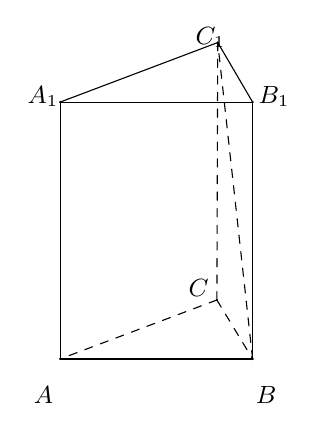
\begin{tikzpicture}[line cap=round,line join=round,font=\small,x=0.03515cm,y=0.03515cm]
% ===== 实线（6 段）=====
\draw (444.0,23.4)--(513.5,23.4);    % AB（底前边）
\draw (444.0,23.4)--(444.0,116.2);   % AA1（左侧棱）
\draw (513.5,23.4)--(513.5,116.2);   % BB1（右侧棱）
\draw (444.0,116.2)--(513.5,116.2);  % A1B1（上底边，源内未画虚线）
\draw (444.0,116.2)--(500.9,137.7);  % A1C1（上底左后边）
\draw (513.5,116.2)--(500.9,137.7);  % B1C1（上底右后边）
% ===== 虚线（4 段）=====
\draw[dashed] (500.9,137.7)--(500.6,44.7);  % C1C（后侧棱）
\draw[dashed] (500.6,44.7)--(444.0,23.4);   % CA（底后左边）
\draw[dashed] (500.6,44.7)--(513.5,23.4);   % CB（底后右边）
\draw[dashed] (513.5,23.4)--(500.9,137.7);  % BC1（所求异面直线之一）
% ===== 顶点实心点（源内六顶点均带小点，直径约 0.9pt）=====
\fill (444.0,23.4) circle[radius=0.45pt];
\fill (513.5,23.4) circle[radius=0.45pt];
\fill (500.6,44.7) circle[radius=0.45pt];
\fill (444.0,116.2) circle[radius=0.45pt];
\fill (513.5,116.2) circle[radius=0.45pt];
\fill (500.9,137.7) circle[radius=0.45pt];
% ===== 标签（照源墨迹中心，显式坐标）=====
\node[anchor=center,inner sep=0] at (438.0,10.5) {\(A\)};
\node[anchor=center,inner sep=0] at (518.4,10.5) {\(B\)};
\node[anchor=center,inner sep=0] at (494.0,49.0) {\(C\)};
\node[anchor=center,inner sep=0] at (437.8,118.3) {\(A_{1}\)};
\node[anchor=center,inner sep=0] at (521.3,118.3) {\(B_{1}\)};
\node[anchor=center,inner sep=0] at (498.3,139.5) {\(C_{1}\)};
\end{tikzpicture}
\end{center}
\nopagebreak[4]
\end{question}
\begin{question}
\gkti{26}（本题满分 8 分）

已知函数 \(f(x)=\sin x+\sqrt{3}\cos x\)，求 \(f(x)\) 的最小正周期及最大值，并指出 \(f(x)\) 取得最大值时 \(x\) 的值．

\Needspace{0.4\textheight}
\end{question}
\begin{question}
\gkti{27}（本题满分 8 分）

如图，汽车前灯反射镜与轴截面的交线是抛物线的一部分，灯口所在的圆面与反射镜的轴垂直，灯泡位于抛物线的焦点 \(F\) 处，已知灯口直径是 \(24\mathrm{cm}\)，灯深 \(10\mathrm{cm}\)，求灯泡与反射镜的顶点 \(O\) 的距离．
\nopagebreak[4]
\begin{center}% 第 27 题前灯抛物面反射镜轴截面图：源为嵌入位图（938×1392），按题设数据等比作图实测
% （1 cm = 5.77 pt；页面坐标 y 向下换算 Y = 490 − y_page）。
% 照源要点：抛物线 y² = 14.4x 精确作图（灯口半径 12 cm 处与椭圆上下端点重合）；
% 灯口圆面画为透视椭圆（纵半轴 = 12 cm，横半轴 14.3 pt，轴比 0.203）；
% 椭圆内竖虚线自中心向下至椭圆下端附近（源内上半段未画）；24cm 竖排标注、10cm 横排标注
% （尺寸线在文字处断开），尺寸线两端向外实心箭头，Times 正体「cm」。
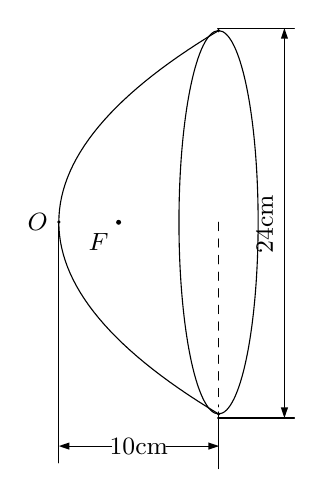
\begin{tikzpicture}[line cap=round,line join=round,font=\small,x=0.03515cm,y=0.03515cm]
% ===== 抛物线（y² = 14.4 x，ξ 以 cm 计，ξ ∈ [−12,12]）=====
\draw plot[domain=-12:12,samples=61,variable=\t] ({441.1+5.77*(\t*\t/14.4)}, {91.6+5.77*\t});
% ===== 灯口透视椭圆（与抛物线两端点重合）=====
\draw (498.8,91.6) ellipse [x radius=14.3, y radius=69.24];
% ===== 椭圆内竖直虚线（自中心向下，照源上半段未画）=====
\draw[dashed] (498.8,91.6)--(498.8,24.9);
% ===== 焦点 F（实心点）与 O 顶点、抛物线-椭圆上下接合处小点（照源）=====
\fill (462.7,91.6) circle[radius=0.9pt];
\fill (441.1,91.7) circle[radius=0.65pt];
\fill (498.8,160.84) circle[radius=0.65pt];
\fill (498.8,22.36) circle[radius=0.65pt];
% ===== 24cm 尺寸线（竖直，两端向外箭头）与上下水平引出线 =====
\draw (498.5,161.7)--(526.2,161.7);   % 上引出线
\draw (498.5,20.9)--(526.2,20.9);     % 下引出线
\draw (522.6,157.9)--(522.6,24.7);    % 尺寸线（两端留箭头位）
\fill (522.6,161.7)--(521.3,157.9)--(523.9,157.9)--cycle;   % 上端向外箭头
\fill (522.6,20.9)--(521.3,24.7)--(523.9,24.7)--cycle;      % 下端向外箭头
% ===== 10cm 尺寸线（水平，文字处断开，两端向外箭头）与竖直引出线 =====
\draw (441.1,91.7)--(441.1,4.7);      % 左竖直引出线（过 O 向下）
\draw (498.8,23.1)--(498.8,2.6);      % 右竖直引出线
\draw (444.9,10.75)--(460.2,10.75);   % 尺寸线左段（留箭头位）
\draw (479.8,10.75)--(495.2,10.75);   % 尺寸线右段（文字处断开）
\fill (441.1,10.75)--(444.9,9.45)--(444.9,12.05)--cycle;    % 左端向外箭头
\fill (498.96,10.75)--(495.16,9.45)--(495.16,12.05)--cycle; % 右端向外箭头
% ===== 标签（照源位置）=====
\node[anchor=center,inner sep=0] at (433.5,91.7) {\(O\)};
\node[anchor=center,inner sep=0] at (455.5,84.5) {\(F\)};
\node[anchor=center,inner sep=0,rotate=90] at (515.5,91.0) {\(24\mathrm{cm}\)};
\node[anchor=center,inner sep=0] at (470.0,10.75) {\(10\mathrm{cm}\)};
\end{tikzpicture}
\end{center}
\nopagebreak[4]
\end{question}
\begin{question}
\gkti{28}（本题满分 12 分）本题共有 2 个小题，第 1 小题满分 4 分，第 2 小题满分 8 分．

已知数列 \(\{a_{n}\}\) 是公差为 2 的等差数列．

（1） 若 \(a_{1}\)，\(a_{3}\)，\(a_{4}\) 成等比数列，求 \(a_{1}\) 的值；

（2） 设 \(a_{1}=-19\)，数列 \(\{a_{n}\}\) 的前 \(n\) 项和为 \(S_{n}\)．数列 \(\{b_{n}\}\) 满足 \(b_{1}=1\)，\(b_{n+1}-b_{n}=\left(\dfrac{1}{2}\right)^{n}\)．记 \(c_{n}=S_{n}+2^{n-1}\cdot b_{n}\)（\(n\in\mathbf{N}^{*}\)），求数列 \(\{c_{n}\}\) 的最小项 \(c_{n_{0}}\)（即 \(c_{n_{0}}\leqslant c_{n}\) 对任意 \(n\in\mathbf{N}^{*}\) 成立）．

\end{question}
\begin{question}
\gkti{29}（本题满分 12 分）本题共有 2 个小题，第 1 小题满分 5 分，第 2 小题满分 7 分．

对于函数 \(f(x)\) 与 \(g(x)\)，记集合 \(D_{f>g}=\{x\mid f(x)>g(x)\}\)．

（1） 设 \(f(x)=2|x|\)，\(g(x)=x+3\)，求 \(D_{f>g}\)；

（2） 设 \(f_{1}(x)=x-1\)，\(f_{2}(x)=\left(\dfrac{1}{3}\right)^{x}+a\cdot 3^{x}+1\)，\(h(x)=0\)．如果 \(D_{f_{1}>h}\cup D_{f_{2}>h}=\mathbf{R}\)，求实数 \(a\) 的取值范围．

\end{question}
\gkpart{第Ⅱ卷（附加题）}

（本卷源内独立编号 1–7：选择题 1–3、填空题 4–6、解答题 7；对应本库连续编号第 30–36 题。）

\gkpart{一、选择题}

（本大题满分 9 分）本大题共有 3 题，每题有且只有一个正确答案，考生应在答题纸的相应编号上，将代表答案的小方格涂黑，选对得 3 分，否则一律得 0 分．

\begin{question}
\gkti{30}若函数 \(f(x)=\sin(x+\varphi)\) 是偶函数，则 \(\varphi\) 的一个值是（　）

\begin{gkopts}(2)
\task （A）0
\task （B）\(\dfrac{\pi}{2}\)
\task （C）\(\pi\)
\task （D）\(2\pi\)
\end{gkopts}

\end{question}
\begin{question}
\gkti{31}在复平面上，满足 \(|z-1|=4\) 的复数 \(z\) 所对应的点的轨迹是（　）

\begin{gkopts}(4)
\task （A）两个点
\task （B）一条线段
\task （C）两条直线
\task （D）一个圆
\end{gkopts}

\Needspace{0.4\textheight}
\end{question}
\begin{question}
\gkti{32}已知函数 \(f(x)\) 的图像是折线段 \(ABCDE\)，如图，其中 \(A(1,2)\)，\(B(2,1)\)，\(C(3,2)\)，\(D(4,1)\)，\(E(5,2)\)，设 \(k\)，\(b\in\mathbf{R}\)，若直线 \(y=kx+b\) 与 \(f(x)\) 的图像恰有 4 个不同的公共点，则 \(k\) 的取值范围是（　）
\nopagebreak[4]
\begin{center}% 第 32 题（源Ⅱ-3）折线段 ABCDE：源为嵌入位图（374×284 @152.3 ppi），
% 按题面坐标等比绘制（1 单位 = 17.87 pt），顶点与标签按源实测（Y = 310 − y_page）。
% 照源要点：两轴仅正方向端有箭头；两轴均越过原点一段（x 轴左伸 3.25 单位、y 轴下伸 2.72 单位，无箭头）；
% 无刻度、无数字；原点与五个顶点各一枚实心点（源内为红点，本项目黑白输出以实心黑点复刻）。
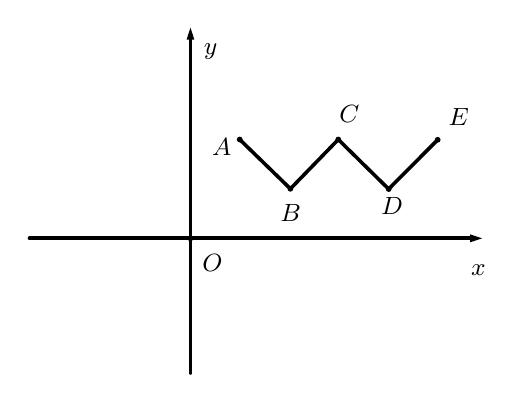
\begin{tikzpicture}[line cap=round,line join=round,font=\small,x=0.03515cm,y=0.03515cm]
% ===== 坐标轴（源线宽约 1.4pt；正方向端实心三角箭头；负方向端无箭头）=====
\draw[line width=1.4pt] (340.3,18.2)--(500.0,18.2);   % x 轴（线体止于箭头基）
\draw[line width=1.4pt] (398.4,-30.4)--(398.4,90.5);  % y 轴
\fill (503.8,18.2)--(499.4,16.75)--(499.4,19.65)--cycle;   % x 轴右端实心箭头
\fill (398.4,94.3)--(397.0,90.0)--(399.8,90.0)--cycle;     % y 轴上端实心箭头
% ===== 折线段（源线宽约 1.3pt）=====
\draw[line width=1.3pt] (416.2,53.9)--(434.5,36.1)--(451.8,53.9)--(470.0,36.0)--(487.7,53.8);
% ===== 实心点（原点与五顶点）=====
\fill (398.4,18.2) circle[radius=1.05pt];
\fill (416.2,53.9) circle[radius=1.05pt];
\fill (434.5,36.1) circle[radius=1.05pt];
\fill (451.8,53.9) circle[radius=1.05pt];
\fill (470.0,36.0) circle[radius=1.05pt];
\fill (487.7,53.8) circle[radius=1.05pt];
% ===== 标签（照源墨迹中心）=====
\node[anchor=center,inner sep=0] at (409.7,51.1) {\(A\)};
\node[anchor=center,inner sep=0] at (434.6,27.2) {\(B\)};
\node[anchor=center,inner sep=0] at (455.8,63.1) {\(C\)};
\node[anchor=center,inner sep=0] at (471.2,30.0) {\(D\)};
\node[anchor=center,inner sep=0] at (495.3,62.2) {\(E\)};
\node[anchor=center,inner sep=0] at (406.4,9.2) {\(O\)};
\node[anchor=center,inner sep=0] at (502.4,6.6) {\(x\)};
\node[anchor=center,inner sep=0] at (405.7,85.8) {\(y\)};
\end{tikzpicture}
\end{center}
\nopagebreak[4]
（A）\((-1,0)\cup(0,1)\)　（B）\(\left(-\dfrac{1}{3},\dfrac{1}{3}\right)\)

（C）\((0,1]\)　（D）\(\left[0,\dfrac{1}{3}\right]\)

\end{question}
\gkpart{二、填空题}

（本大题满分 9 分）本大题共有 3 小题，考生应在答题纸相应编号的空格内直接填写结果，每个空格填对得 3 分，否则一律得 0 分．

\begin{question}
\gkti{33}椭圆的 \(\dfrac{x^{2}}{25}+\dfrac{y^{2}}{9}=1\) 的长半轴的长为\gkblank{}．

\end{question}
\begin{question}
\gkti{34}已知圆锥的母线长为 10，母线与轴的夹角为 \(30^{\circ}\)，则该圆锥的侧面积为\gkblank{}．

\end{question}
\begin{question}
\gkti{35}小明用数列 \(\{a_{n}\}\) 记录某地区 2015 年 12 月份 31 天中每天是否下过雨，方法为：当第 \(k\) 天下过雨时，记 \(a_{k}=1\)；当第 \(k\) 天没下过雨时，记 \(a_{k}=-1\)（\(1\leqslant k\leqslant 31\)）．他用数列 \(\{b_{n}\}\) 记录该地区该月每天气象台预报是否有雨，方法为：当预报第 \(k\) 天有雨时，记 \(b_{k}=1\)；当预报第 \(k\) 天没有雨时，记 \(b_{k}=-1\)（\(1\leqslant k\leqslant 31\)）．记录完毕后，小明计算出 \(a_{1}b_{1}+a_{2}b_{2}+a_{3}b_{3}+\cdots+a_{31}b_{31}=25\)，那么该月气象台预报准确的总天数为\gkblank{}．

\end{question}
\gkpart{三、解答题}

（本大题满分 12 分）解答本题必须在答题纸相应编号的规定区域内写出必要的步骤．

\begin{question}
\gkti{36}（本题满分 12 分）本题共有 2 个小题，第 1 小题满分 4 分，第 2 小题满分 8 分．

对于数列 \(\{a_{n}\}\) 与 \(\{b_{n}\}\)，若对数列 \(\{c_{n}\}\) 的每一项 \(c_{k}\)，均有 \(c_{k}=a_{k}\) 或 \(c_{k}=b_{k}\)，则称数列 \(\{c_{n}\}\) 是 \(\{a_{n}\}\) 与 \(\{b_{n}\}\) 的一个“并数列”．

（1） 设数列 \(\{a_{n}\}\) 与 \(\{b_{n}\}\) 的前三项分别为 \(a_{1}=1\)，\(a_{2}=3\)，\(a_{3}=5\)，\(b_{1}=1\)，\(b_{2}=2\)，\(b_{3}=3\)，若 \(\{c_{n}\}\) 是 \(\{a_{n}\}\) 与 \(\{b_{n}\}\) 的一个“并数列”，求所有可能的有序数组 \((c_{1},c_{2},c_{3})\)；

（2） 已知数列 \(\{a_{n}\}\)，\(\{c_{n}\}\) 均为等差数列，\(\{a_{n}\}\) 的公差为 1，首项为正整数 \(t\)；\(\{c_{n}\}\) 的前 10 项和为 \(-30\)，前 20 项和为 \(-260\)，若存在唯一的数列 \(\{b_{n}\}\)，使得 \(\{c_{n}\}\) 是 \(\{a_{n}\}\) 与 \(\{b_{n}\}\) 的一个“并数列”，求 \(t\) 的值所构成的集合．

\end{question}